% Paper template for TAR 2018
% (C) 2014 Jan Šnajder, Goran Glavaš, Domagoj Alagić, Mladen Karan
% TakeLab, FER

\documentclass[10pt, a4paper]{article}

\usepackage{tar2018}

\usepackage[utf8]{inputenc}
\usepackage[pdftex]{graphicx}
\usepackage{booktabs}
\usepackage{amsmath}
\usepackage{amssymb}

%\title{Making your deep neural network's life burden free}
%\title{Supercharged deep learning -- in pursuit of the tiniest model}
\title{Littlest teeniest tiniest supercharged deep learning model}

\name{David Lozić, Luka Markušić} 

\address{
University of Zagreb, Faculty of Electrical Engineering and Computing\\
Unska 3, 10000 Zagreb, Croatia\\ 
\texttt{\{david.lozic,luka.markusic\}@fer.hr}\\
}
          
         
\abstract{ 
  This paper describes the system we used to find a lightweigt
  model which offers acceptable results with fast performance.
  To do this we constructed a basic grid search framework which
  was trained on English version of the 2018 SemEval Task 1 
  Emotion Intensity Regression dataset.
  Our system was evaluated on the official competition test set,
  and performed surprisingly well given it's small size.
}

\begin{document}

\maketitleabstract

\section{Introduction}

Sentiment analysis might be more commonly known by its flashier and broader title, \textit{opinion mining}. 
Generally speaking, the task of sentiment analysis is to identify and categorize the writer's feelings and/or opinions into several categories. 
It has become critical for companies to see how customer's opinions change with the passage of time and trends. 
In the academia, the very popular SemEval series hosts many sentiment analysis competitions annually, with many different subtasks.

In recent years, the trend seems to follow deep learning models,
as they often occupy the top positions on the leaderboards.
At the very top of these competitions many elaborate models 
and complex ensambles can be found
which often provide a minor boost in performance.
Given that these models provide satisfactory performance,
we are interested in finding the minimal working model architecture
which still offers acceptable results.
The motivation behind this is to find the optimal industry oriented
model which would work well in a production environment.

This is made possible due to the rather small size of the dataset,
which provides us with the unique opportunity to do a detailed
architecture and hyperparameter analysis.
In essence, we perform an architecture and hyperparameter grid
search in pursuit of a lightweight model.

\section{Related work}
A substantial number of approaches rely greatly on an underlying sentiment lexicon \citep{lexicon_paper} which, while being one of the most robust, is one of the most time-consuming methods. The trend regarding models based on word representations as vectors of real numbers \citep{w2v} shows no inclination to slow down. Our main source of inspiration was EiTAKA's system \citep{mohammed-semeval} for SemEval-2018. The task their model was suited for was comprised of several different problems:

\textbf{EI-reg:} given a tweet and an emotion, determine the intensity of that emotion as a score between 0 and 1.

\textbf{EI-oc:} given a tweet and an emotion, classify the tweet into one of four ordinal classes of intensity.

\textbf{V-reg:} given a tweet, determine the valence of a tweet as a score between 0 and 1.

\textbf{V-oc:} given a tweet, classify it into one of seven ordinal classes.


Their work was focused towards reaching the best results, as for our proposed model builds upon their work, trying to strip down all the unnecessary material while preserving performance.

\section{Resources}
The dataset for all of the tasks was provided by SemEval itself \citep{mohammed-semeval}, both in English, Spanish and Arabic, our language of choice was English. Additional resources in form of word embeddigs and sentiment lexicons were provided by Stanford \citep{glove} and National Research Council in Canada \citep{nrcic}, respectively. 

In order to stay in the mindset of trying to obtain a lightweight model, we've limited the word embeddings to 200 dimensional vectors, and only one sentiment lexicon will be used.


\section{System Description}
In this section we present how our system performs the grid search.
The system has been implemented using the Keras deep learning library \citep{chollet2015keras}.

\subsection{Preprocessing}
For text preprocessing, we use the tokenizer tool provided in the Keras library.
The tweets are lowercased and the special characters and
punctuations are removed.
These characters include: \textit{!"#\$\%&()*+,-./:;<=>?@[\textbackslash]\^\_`\{|\}~}.

After this normalization step, the tweets are tokenized using the Keras tokenizer.

\subsection{Input}
The words from the preprocessing step are mapped to word embeddings
and affect embeddings.
For word embeddings, we use the GloVe word vectors \citep{glove} 
which embed words into 200 dimensional vectors trained on the Twitter corpora,
on 2B tweets in total.
The affect embedding map words to the affect values which are
extracted from the NRC affect lexicon \citep{mohammed-semeval}
which were also trained on the Twitter corpora. The lexicon consists of 6000 words in total, out of each word may represent multiple emotions.
These embeddings produce 4 dimensional word vectors where every
dimension represents an affect intensity value for the following emotions: \textit{anger, fear, joy, sadness}.
Finally, the two embeddings are concatenated into a single 204 dimension embedding.
These embeddings represent the model input.

\subsection{Architecture grid}
The system performs hyperparameter search for all architectures
given by the user. 
An architecture is defined by a list of layers from which
the model is built using the \textit{Sequential} Keras API.
En example architecture can be seen in Figure 1.
The system fills every layer of the architecture with
arguments generated from the hyperparameter grid.
The sequential list structure of architectures does not
allow for more complex models with multiple inputs that can be
compiled using the \textit{Functional} Keras API.
But this was not our goal since we are searching for minimal models, 
although the system could be easily modified to satisfy such a need.

\subsection{Hyperparameter grid}
To perform hyperparameter search, the user needs to define
a list of possible values for chosen parameters of every type
of layer which is present in the architecture.
The system creates a Cartesian product of hyperparameters
which are used to fill the layers of the specified architecture.

\begin{figure}
\begin{center}
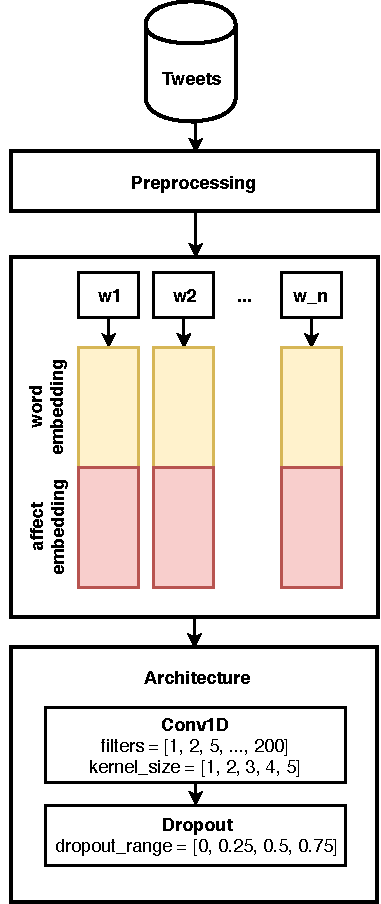
\includegraphics[width=0.7\columnwidth]{images/architecture.pdf}
\caption{Model pipeline with an example architecture.}
\label{fig:figure1}
\end{center}
\end{figure}


\subsection{Training}
The model has been trained using the Adam optimizer with the following values:
\texttt{Adam(lr=0.001, beta1=0.9, beta2=0.999, epsilon=None, decay=0.0, amsgrad=False)}
Since the dataset is small, the optimizer often does not converge for larger models.
To combat this, we perform a variant of k-fold cross validation.


\section{Results}
Our experimentation showed interesting results. 
From the architecture and parameter grid, we chose 3 models for representation.

The first model, which we dub the \textit{Minimal Convnet}, is as follows:
\texttt{[Conv1D(2, 1), BatchNormalization, Dropout(0.25)]}.

The second \textit{Small Convnet} is represented as: 
\texttt{[Conv1D(10, 3), BatchNormalization, Dropout(0.5)]}, and the third 
\textit{Best Convnet} as: 
\texttt{[Conv1D(100, 3), BatchNormalization, Dropout(0.75)]}.
The results are presented in Table 1.
Surprisingly, the Minimal Convnet with its measly two filters 
and kernel size 1 holds up admirably, scoring
better results than the SVM baseline, but falling far behind the 
previous work.
The Small Convnet is our model of choice, which achieves solid 
performance while maintaining a very small architecture.
This size of convolutional network seems to be the sweet spot in our testing.
Further increasing the model size only leads to worse performance and 
harder training.
Although this model still falls behind the EiTAKA considerably, their
implementation uses multiple word embeddings, multiple semantic lexicons,
a much larger convolutional model with multiple channels combined with an
XGBoost regressor into an ensemble.
In the face of adversity, our Small Convnet holds its own.


\begin{table}
\caption{Task 1.a results (emotion intensity regression)}
\label{tab:narrow-table}
\begin{center}
\begin{tabular}{lllll}
\toprule
& joy & anger & fear & sadness \\
\midrule
EiTAKA    & 0.723  & 0.704 & 0.715 & 0.731 \\
Best Convnet & 0.634 & 0.605 & 0.611 & 0.627 \\
Small Convnet & 0.627 & 0.603 & 0.612 & 0.621 \\
Minimal Convnet & 0.587 & 0.573 & 0.569 & 0.591 \\
SVM unigrams baseline & 0.526 & 0.525 & 0.575 & 0.453 \\
Random baseline & -0.018 & 0.024 & -0.058 & 0.020 \\
\bottomrule
\end{tabular}
\end{center}
\end{table}


\section{Conclusion}
This work focused on finding the smallest viable model for the task of affect detection.
To do this, we used the data provided in the first task of the SemEval 2018 competition.
We created a basic framework for grid searching deep learning
models and hyperparameters, and performed an extensive search in pursuit
of the smallest model with acceptable performance.
Our brave little models performed admirably in the face of great adversity.
While they did not match the giants at the very top of the leaderboards, 
they did prove to be competitive in their own right.

In future work, it would be wise to find a richer sentiment lexicon
than the affect lexicon we used. 
Despite our initial hopes, the semantic lexicon more often than not failed 
to offer values for given tokens since many of them were not a part of the 
relatively small vocabulary. None the less, it doesn't add a lot of overhead, 
and we believe that it would improve the model significantly.
%While the lexicon is well structured for our needs, 
%the percentage of matched words is very low, and we believe
%that would improve the model significanlty with little overhead.




\bibliographystyle{tar2018}
\bibliography{tar2018} 

\end{document}

